\documentclass[12pt]{article}
\usepackage{titling}
\usepackage[absolute]{textpos}
\setlength{\TPHorizModule}{10mm}
\setlength{\TPVertModule}{10mm}
\usepackage[top=2.5cm, bottom=2.5cm, left=3cm, right=2.5cm]{geometry}
\usepackage[polish]{babel}
\usepackage{polski}
\usepackage[utf8]{inputenc}
\usepackage{graphicx}
\usepackage{floatrow}
\usepackage{listings}
\usepackage{color}
\linespread{1.5}
\title{Narzędzie wspomagające tworzenie ciągów przetwarzania wideo w oparciu o bibliotekę GStreamer}
\author{Marcin Kolny}
\usepackage[T1]{fontenc}
\usepackage{helvet}
\renewcommand*{\familydefault}{\sfdefault}
\renewcommand{\maketitle}{
  \begin{titlepage}
    \begin{figure}  
      
\includegraphics[width=40mm]{img/polsl-logo.png}
    \end{figure}
    \begin{center}
      \begingroup
      \fontsize{18pt}{21pt}\selectfont
      \textbf{Politechnika Śląska\\
        Wydział Automatyki, Elektroniki i Informatyki\\
        Kierunek Informatyka}\\
      \vspace{22mm}
      Projekt inżynierski\\
      \vspace{22mm}
      \endgroup
      \begingroup
      \fontsize{14pt}{17pt}\selectfont
      \thetitle \\
      \endgroup
      \vspace{30mm}
    \end{center}
    \begin{textblock}{14}(2.5,21.5)
      \fontsize{14pt}{17pt}\selectfont
      Autor: \theauthor \\
      Kierujący pracą: dr Ewa Lach\\
    \end{textblock}
    \begin{textblock}{20}(2.5,26.5)
      \fontsize{14pt}{17pt}\selectfont
      Gliwice, styczeń 2014\\
    \end{textblock}

  \end{titlepage}
}
\begin{document}
\definecolor{cppred}{rgb}{0.6,0,0} % strings
\definecolor{cppgreen}{rgb}{0.25,0.5,0.35} % comments
\definecolor{cpppurple}{rgb}{0.5,0,0.35} % keywords
\definecolor{cppblue}{rgb}{0.25,0.35,0.75} % doxygen
\definecolor{lightgrey}{rgb}{0.9,0.9,0.9}
\lstset{language=C++,
basicstyle=\ttfamily,
keywordstyle=\color{cpppurple}\bfseries,
stringstyle=\color{cppred},
commentstyle=\color{cppgreen},
morecomment=[s][\color{cppblue}]{/**}{*/},
numbers=left,
backgroundcolor=\color{lightgrey},
numberstyle=\tiny\color{black},
stepnumber=1,
numbersep=10pt,
tabsize=4,
showspaces=false,
showstringspaces=false}
\maketitle
\tableofcontents
\cleardoublepage
\section{Analiza problemu}
\subsection{Narzędzia}
\subsubsection{Biblioteka GStreamer}
\paragraph{}
Biblioteka GStreamer służy do konstruowania grafów przetwarzania strumieni multimedialnych. Biblioteka została napisana w języku ANSI C i dostępna jest pod systemami Linux, Windows, OS X oraz Android.

GStreamer wydany jest na licencji GNU GPL i może być wykorzystywany w zastosowaniach komercyjnych. Licencja pozwala również na modyfikowanie i dystrybucję kodu źródłowego biblioteki.
Biblioteka oferuje użytkownikowi wiele gotowych elementów do przetwarzania wideo (np. enkodery czy dekodery audio-video), do generowania sygnałów multimedialnych, a także do prezentacji wyników użytkownikowi. Ponadto, istnieje możliwość pisania własnych elementów, które można następnie użyć w bilbliotece GStreamer.

Biblioteka GStreamer oparta jest o \textbf{elementy} (ang. \textit{elements}). Elementem nazywany jest obiekt, który realizuje zadany algorytm. Przykładowym elementem jest dekoder, którego celem jest dekodowanie strumienia multimedialnego o zadanym formacie.

Element może zawierać gniazda, dzięki którym możliwe jest połączenie go z innymi elementami.

Elementy dzielą się na te, które zawierają tylko gniazda wejściowe (ang. \textit{sink elements}), które posiadają tylko gniazda wejściowe (ang. \textit{source elements}), oraz elementy zawierające zarówno gniazda wejściowe, jak i wyjściowe (ang. \textit{filter elements}).
\begin{figure}[H]
  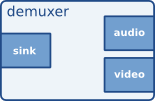
\includegraphics[width=40mm]{img/sample-demuxer.png}
  \caption{Przykładowy element typu \textit{demuxer} \cite{gstmainpage}}
  \label{fig:sampleDemuxer}
\end{figure}
\paragraph{}
Rysunek ~\ref{fig:sampleDemuxer} przedstawia przykładowy element, zawierający dwa gniazda wyjściowe, i jedno gniazdo wejściowe (jest to szczególny wariant filtra, tzw. \textit{demuxer}).
\paragraph{}
\textbf{Kontener} (ang. \textit{bin}) jest szczególnym elementem. Podobnie, jak elementy, kontenery posiadają gniazda. Natomiast algorytmy zdefiniowane w elemencie-kontenerze realizowane są poprzez inne elementy, które agregowane są w danym kontenerze. Rysunek ~\ref{fig:sampleBin} przedstawia przykładowy kontener, zawierający dwa elementy, oraz jedno gniazdo wejściowe.
\begin{figure}[H]
  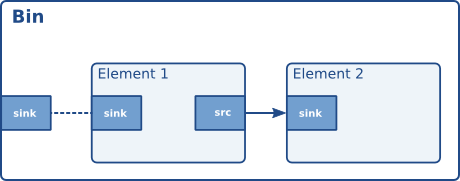
\includegraphics[width=100mm]{img/sample-bin.png}
  \caption{Przykładowy kontener \cite{gstmainpage}}
  \label{fig:sampleBin}
\end{figure}
\paragraph{}
\textbf{Strumień} (ang. \textit{pipeline}) jest specjalnym przypadkiem kontenera. Jest to kontener nadrzędny całego modelu programu. Przechowuje w sobie główne elementy oraz kontenery agregujące inne obiekty przetwarzające. Strumień nie posiada żadnych gniazd. Rysunek ~\ref{fig:samplePipeline} przedstawia przykładowy strumień, realizujący operację odtwarzania strumienia audio-video z pliku ogg.
\begin{figure}[H]
  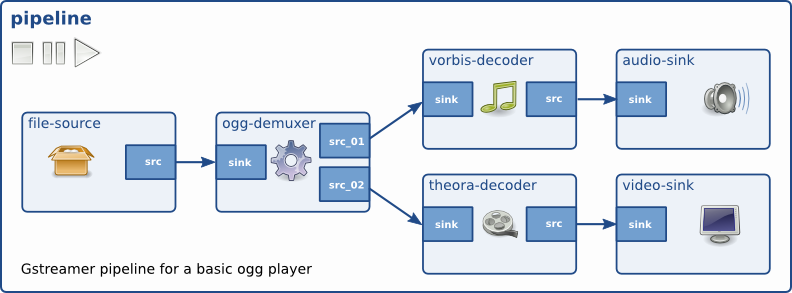
\includegraphics[width=150mm]{img/simple-player.png}
  \caption{Przykładowy strumień \cite{gstmainpage}}
  \label{fig:samplePipeline}
\end{figure}
\paragraph{}
\textbf{Gniazda} (ang. \textit{pads}) to obiekty umożliwiające połączenie ze sobą dwóch różnych elementów. Gniazdo charakteryzuje się dwoma właściwościami: kierunkiem oraz dostępnością. Pod względem kierunku, gniazda podzielone są na dwie grupy:
\begin{itemize}
 \setlength{\itemsep}{0em}
  \item wejściowe (ang. \textit{sink pads}),
  \item wyjściowe (ang. \textit{src pads}).
\end{itemize}

Gniazda wyjściowe (źródłowe), służą do przesyłania danych do następnego elementu. Gniazda wejściowe wykorzystywane są natomiast do odbierania danych przesłanych z poprzednich elementów.

Kolejna właściwość, dzieli zbiór gniazd na trzy grupy:
\begin{itemize}
 \setlength{\itemsep}{0em}
  \item występujące zawsze (ang. \textit{always pads}),
  \item występujące w zależności od danych (ang. \textit{sometimes pads, dynamic pads}),
  \item pojawiające się na żądanie użytkownika (ang. \textit{request pads}).
\end{itemize}

Gniazda należące do pierwszej grupy występują zawsze w elemencie, i nie można ich usunąć.
Druga grupa gniazd, to takie, które pojawiają się tylko wtedy, kiedy wystąpi taka potrzeba. Na rysunku ~\ref{fig:requestPadsDemux} pokazane zostały dwa demultiplexery połączone z elementem wczytującym dane z pliku. W pierwszym przypadku (po lewej), w pliku zapisane zostały dwa strumienie multimedialne, dla tego element \textit{ogg-demuxer} zawiera dwa gniazda źródłowe. W drugim przypadku (po lewej), plik zawiera tylko jeden strumień multimedialny, stąd demuxer wygenerował tylko jedno gniazdo.
\begin{figure}[H]
  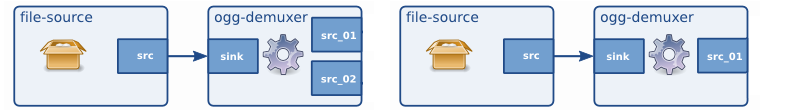
\includegraphics[width=150mm]{img/request-pads-demux.png}
  \caption{Dynamiczne gniazda elementu demuxera \cite{gstmainpage}}
  \label{fig:requestPadsDemux}
\end{figure}
Ostatnia grupa, to gniazda, pojawiające się na żądanie użytkownika. Można wyobrazić sobie odwrotną sytuację do opisywanej w poprzednim akapicie. Użytkownik wstawia element muxera, który łączy kilka strumieni. W zależności od tego, ile strumieni użytkownik będzie chciał połączyć, tyle żądań o gniazdo wejściowe będzie musiał zgłosić.

\textbf{Połączenia} (ang. \textit{links}) pomiędzy dwoma elementami odbywają się przez tzw. \textit{negocjacje}. Każde gniazdo elementu posiada właściwość określającą, jakiego typu dane akceptuje dane gniazdo. Właściwości te nazywane są możliwościami (ang. \textit{capabilities}, \textit{caps}). Proces negocjacji ma na celu odnalezienie wspólnego formatu danych, jaki może zostać zaakceptowany przez odybwa gniazda (gniazdo wejściowe oraz wyjściowe), które użytkownik chce ze sobą połączyć. Jeśli negocjacje zakończą się niepowodzeniem (to znaczy, nie uda się znaleźć wspólnego formatu), połączenie nie zostanie wykonane.

\subsubsection{Adapter C++ - gstreamermm}
\paragraph{}
Adapter (ang. \textit{wrapper}) jest wzorcem projektowym, który ma na celu uwspólnienie interfejsu pomiędzy dwoma blokami kodu źródłowego. Biblioteka GStreamer została napisana w języku ANSI C, dla tego, aby umożliwić programistom innych języków korzystanie z biblioteki, nie mieszając różnych języków, powstało kilka adapterów dla innych języków programowania (np. C++ czy C\#).

\textbf{gstreamermm} to projekt, którego celem jest stworzenie biblioteki-adaptera w języku C++ dla biblioteki GStreamer. Projekt rozwijany jest na licencji LGPL, dla tego każdy może uzyskać dostęp do kodu źródłowego biblioteki, a także w dowolny sposób modyfikować źródła.

Biblioteka gstreamermm należy do rodziny projektów pochodzących od \textbf{gtkmm}. Projekty te opierają się głównie o generowanie kodu źródłowego w języku C++ na podstawie źródeł napisanych w języku ANSI C. Wszystkie projekty korzystają ze wspólnych generatorów kodu.

Kod źródłowy biblioteki jest w większości \textit{autogenerowany} na podstawie źródeł projektu GStreamer w trójetapowym procesie. Rysunek ~\ref{fig:mmGenerateProcess} prezentuje wszystkie trzy kroki procesu generacji kodu źródłowego.
\begin{figure}[H]
  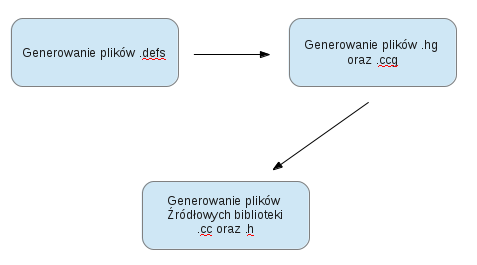
\includegraphics[width=100mm]{img/mm-generate-process.png}
  \caption{Schemat procesu generacji kodu źródłowego biblioteki gstreamermm}
  \label{fig:mmGenerateProcess}
\end{figure}
\begin{enumerate}
 \setlength{\itemsep}{0em}
  \item Pierwszym etapem generacji kodu jest przeszukanie źródeł biblioteki GStreamer, a następnie wygenerowanie plików definicji. Pliki definicji zawierają informacje na temat typów wyliczeniowych zdefiniowanych w bibliotece, funkcji, sygnałów, metod wirtualnych czy struktur danych. W przypadku wygenerowanie przez generator błędnej definicji, stosowane są pisane przez programistę tzw. \textit{łatki} (ang. \textit{patch}).
  \item W kolejnym przebiegu, generator na podstawie plików definicji, generuje pliki \textit{.hg} oraz \textit{.ccg}. Zawartość plików przypomina składnią język C++, jednak zawiera wywołania makrodefinicji ułatwiających adaptowanie poszczególnych elementów biblioteki. Przykład użycia makrodefinicji przedstawiony został na listingu ~\ref{macroSampleUsage}.
Listę dostępnych makr można znaleźć w dokumentacji projektu gnome \cite{devgnomepage}.
    \begin{lstlisting}[caption=Przykład użycia makrodefinicji w pliku \textit{.hg}, label=macroSampleUsage]
_WRAP_METHOD(bool load_preset(const Glib::ustring& name), 
      gst_preset_load_preset)
    \end{lstlisting}
    W przypadku, gdy plik \textit{.hg} zostanie niepoprawnie wygenerowany, programista zmuszony jest do ręcznego napisania tego pliku. W tym wypadku nie stosuje się łatek, ponieważ w większości przypadków, błąd obejmuje większą część pliku, a nie pojedyncze linie.
  \item Ostatni etap generacji kodu źródłowego, to przekształcenie plików \textit{.hg} oraz \textit{.ccg} w pliki źródłowe języka C++. Na przykład, pokazane na listingu ~\ref{macroSampleUsage} zostanie zastąpione kodem zaprezentowanym na listingu ~\ref{outMacroSampleUsage}.
    \begin{lstlisting}[caption=Kod źródłowy wygenerowany na podstawie makrodefinicji, label=outMacroSampleUsage]
bool load_preset(const Glib::ustring& name);
...
bool Preset::load_preset(const Glib::ustring& name)
{
  return gst_preset_load_preset(gobj(), name.c_str());
}
    \end{lstlisting}
    Funkcja \textit{gst\_preset\_load\_preset} jako drugi argument, przyjmuje wartość typu \textit{gchar*}. Generator wiedział, w jaki sposób dokonać konwersji na ten typ z typu \textit{const Glib::ustring\&}. Baza wiedzy, dotycząca konwersji pomiędzy typami ANSI C a typami języka C++, znajduje się w osobnych plikach, pisanych przez programistę.
W tym etapie, wygenerowany kod źródłowy jest zawsze poprawny. Programista może jedynie dopisać dodatkowe pliki. Przechowują one na ogół klasy usprawniające (ale nie rozszerzające funkcjonalność) pracę z biblioteką.
\end{enumerate}

\cleardoublepage
\begin{thebibliography}{9}

\bibitem{gstmainpage}
  http://gstreamer.freedesktop.org, 2013
\bibitem{devgnomepage}
  https://developer.gnome.org, 2013

\end{thebibliography}
\end{document}
